\section{Część obliczeniowa (,,wyższego poziomu'')}
\label{sec:czesc-wyzsza}

Aby zapewnić jak najlepszą realizację zadań postawionych przed częścią obliczeniową, należało wybrać odpowiednie oprogramowanie używane przez ten poziom aplikacji. Przyjęto dwa podstawowe założenia co do niego:
\begin{itemize}
    \item powinna być napisana w języku programowania Python,
    \item powinna używać biblioteki Tango Controls jako swojej podstawy.
\end{itemize}

Pierwsze założenie zostało przyjęte ze względu na niewątpliwe zalety tego języka. Jest on mocno zorientowany na programowanie obiektowe, posiada przejrzystą, nieskomplikowaną składnię oraz, jako język interpretowany, umożliwia szybkie prototypowanie i korzystanie z interaktywnego wiersza poleceń.

Dodatkowo jest to język dostępny w całości na otwartej licencji, a społeczność skupiona wokół niego dostarcza wielu bibliotek ogólnego i szczególnego zastosowania, które również często są otwartym oprogramowaniem. Podjęto w związku z tym próbę znalezienia wśród tych bibliotek takich, które byłyby pomocne w rozwiązywaniu zagadnień optymalizacji dynamicznej - więcej na ten temat w sekcji \ref{sub:czesc-wyzsza-wybor}.

Drugie założenie zostanie wyjaśnione w kolejnej sekcji.

%-------------------------------------------------
\subsection{Opis systemu Tango Controls}
\label{sub:czesc-wyzsza-tango}

Tango Controls to zestaw narzędzi służący do zarządzania rozproszonymi systemami sterowania umożliwiający przyłączanie dowolnych urządzeń oraz fragmentów oprogramowania do jednej magistrali programowej. Jest on również dystrybuowany na otwartej licencji (tzw. słabszej powszechnej licencji publicznej GNU - ang. \emph{Lesser GNU Public Licence} - w wersji 3) i utrzymywany przez konsorcjum placówek naukowych z całej Europy (więcj informacji w \cite{TangoWebsite}).


\subsubsection{Ogólne założenia systemu}
Początki tego oprogramowania sięgają roku 1999, kiedy to w Europejskim Ośrodku Synchrotronu Atomowego w Grenoble podjęto próbę implementacji nowego systemu pozwalającego na połączenie wszystkich urządzeń jedną magistralą programową i zaczęto pracę nad jej uogólnieniem, aby mogła przyjąć dowolny sprzęt, który tylko będzie miał napisany odpowiedni do niej sterownik. Osiągnięto ten cel dzięki użyciu odpowiedniej technologii komunikacyjnej (oryginalnie implementacji architektury CORBA, od wersji 7 również biblioteki ZeroMQ) oraz zastosowaniu własnego protokołu oraz ogólnej przestrzeni adresowej dla wszystkich urządzeń w systemie. Zastosowano tutaj również podejście ,,klient - serwer'', a więc istnieje wyraźne rozgranicznie między interfejsem dla klienta (aplikacji pobierającej dane z systemu) oraz serwera (aplikacji dostarczającej dane). Dostępne są 3 tryby komunikacji między klientami a serwerami:
\begin{itemize}
    \item synchroniczny,
    \item asynchroniczny,
    \item zdarzeniowy.
\end{itemize}

Przyłączanie nowego sprzętu do tego systemu opiera się na zasadzie opakowywania istniejącego kodu służącego do komunikacji z nim kodem realizującym operacje związane z systemem Tango Controls. W związku z tym, że jednym z podstawowych założeń tego systemu jest obiektowość, to opakowanie będzie miało postać \emph{klasy urządzeń}.
Dzięki temu przejmuje on wszystkie zalety (oraz pułapki) programowania obiektowego: możliwość dziedziczenia między klasami, co ułatwia utrzymywanie hierarchicznej struktury pisanego oprogramowania, jak i możliwość współdzielenia bardziej ogólnych klas między różnymi systemami, które korzystają z Tango Controls. W szczególności wszystkie klasy muszą dziedziczyć po bazowej klasie - \emph{Device}.

\subsubsection{Urządzenia i ich serwery}
Podstawowym pojęciem opisywanego systemu jest \emph{urządzenie}, które jest obiektem w sensie programistycznym (instancją klasy danego typu urządzeń). Może to być:
\begin{itemize}
    \item logiczna abstrakcja istniejącego fizycznie sprzętu, niezależnie od tego, czy jest to jeden prosty czujnik, czy bardziej skomplikowane urządzenie z własnym HMI (ang. \emph{Human-Machine Interface}: interfejs człowiek-maszyna),
    \item logiczna abstrakcja grupy urządzeń, również niezależnie od ich stopnia skomplikowania,
    \item fragment oprogramowania - mówi się wtedy o czysto programowym urządzeniu.
\end{itemize}

Definicja przestrzeni adresowej systemu zakłada, że każde urządzenie w systemie ma nazwę składającą się z 3 członów przedzielonych prawymi ukośnikami (,,/''):
\begin{itemize}
    \item domeny,
    \item rodziny,
    \item członka.
\end{itemize}
Przykładowa nazwa wygląda następująco: \texttt{sys/tg\_test/1}.

Dodatkowo podając nazwę urządzenia, można również podać adres bazowy systemu, czyli adres i port, na którym można nawiązać komunikację TCP/IP z urządzeniem zarządzającym dostępem do warstwy persystencji systemu - bazy danych MySQL. Tam przechowywane są informacje na temat urządzeń kiedykolwiek uruchomionych w systemie. Taki adres bazowy systemu określa się jako zmienną środowiskową w systemie operacyjnym o nazwie \texttt{TANGO\_HOST}. Określenie takiej pary adresu i portu jednoznacznie definiuje, z którym systemem zarządzanym przez Tango Controls klient się chce połączyć. Uzupełniona o nią (i o nazwę protokołu) przykładowa nazwa urządzenia wygląda następująco: \texttt{tango://tango-host.org:10000/sys/tg\_test/1}.

Urządzenia systemu Tango są grupowane w \emph{serwery urządzeń} - procesy w systemie operacyjnym, które przy swoim starcie pytają warstwy persystencji o to, jakie urządzenia mają uruchomić. Każdy serwer urządzeń ma określony zestaw klas urządzeń, których instancjami może zarządzać: uruchamiać je, edytować, wyłączać, kasować itp. Umożliwia on również włączenie odpytywania konkretnego elementu interfejsu urządzenia z okresem zadanym w milisekundach. Proponuje się rozróżnienie na klasę urządzeń i typ serwera urządzeń, aby uniknąć nieścisłości. Każdy serwer jest również obiektem klasy urządzeń \emph{DServer}, a jego typ określa to, jakimi klasami urządzeń dysponuje.

Na interfejs urządzenia składają się cztery typy pól w klasie tego urządzenia:
\begin{enumerate}
    \item Atrybuty (ang. \emph{attributes}) - reprezentują wielkości fizyczne, zmieniające się w czasie działania urządzenia. Muszą mieć zdefiniowany typ (jeden z podstawowych typów danych numerycznych lub ciągu znaków) oraz wymiar (Tango Controls obsługuje atrybuty skalarne, wektorowe i macierzowe). Każde urządzenie musi mieć przynajmniej 2 atrybuty: stan i status (testowy opis tego, co się dzieje z urządzeniem). Przykładowy atrybut urządzenia będącego odwzorowaniem silnika krokowego w systemie Tango to pozycja (zmiennoprzecinkowa wartość skalarna) lub stan wyłączników krańcowych (dwuelementowy wektor wartości logicznych).
    
    \item Strumienie (ang. \emph{pipe} - pozwalają na przesyłanie dowolnego typu surowych danych do urządzenia lub na jego zewnątrz. Dla każdej ich paczki trzeba jednak określić ten typ przed transmisją. Mogą być jedno- lub dwukierunkowe. Jest to nowy typ pola w klasach urządzeń, obecny od wersji 9.
    
    \item Komendy (ang. \emph{commands})- będące operacjami, których wykonanie urządzenie umożliwia. Mogą być wywoływane z maksymalnie jednym argumentem wejściowym i również tylko jeden argument wyjściowy mogą zwracać. Przykładem komendy urządzenia będącego logiczną abstrakcją silnika krokowego jest operacja bazowania - znalezienie określonej pozycji sprzężonego enkodera i wyzerowanie rejestru położenia.
    
    \item Właściwości (ang. \emph{properties}) - zawierające statyczną konfigurację urządzenia. Jako jedyne są przechowywane w bazie danych, skąd serwer urządzeń przy starcie pobiera ich wartości.
\end{enumerate}

\begin{figure}[tph]
    \centering
    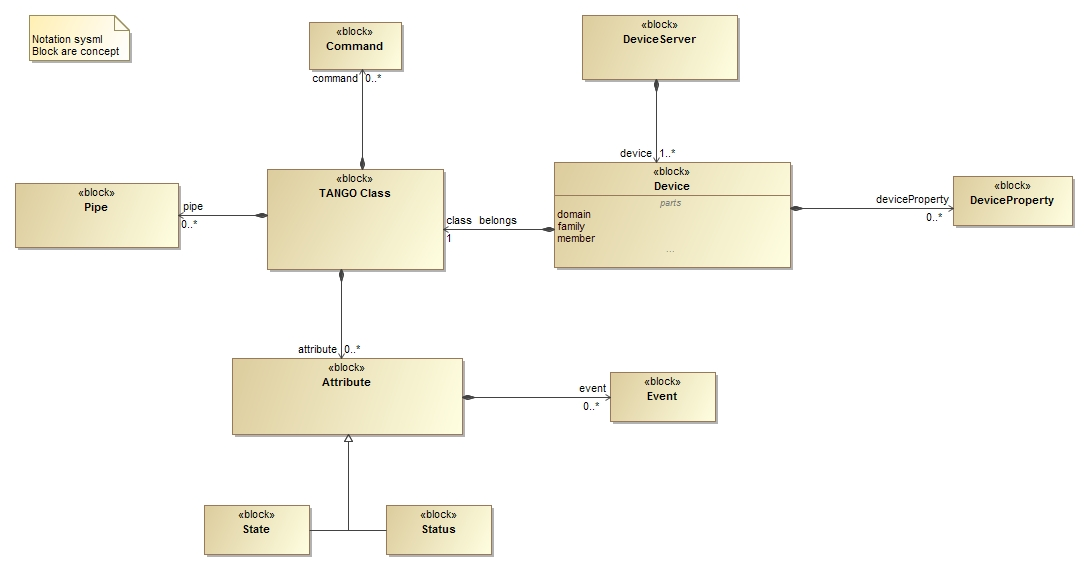
\includegraphics[width=\textwidth]{Grafika/tango_model}
    \caption{Uproszczony model obiektów w systemie Tango Controls. Źródło: \cite{TangoDocs}.}
    \label{fig:tango-model}
\end{figure}

Klasa urządzeń może zawierać definicję maszyny stanów, która opisuje warunki przejść między dowolnymi z 14 dostępnych stanów. Są w tym zbiorze ogólne stany opisujące poprawne działanie urządzenia (INIT, ON, OFF, STANDBY, RUNNING, MOVING), błędy w funkcjonowaniu (ALARM, FAULT, DISABLE), takie nadające się tylko dla określonych typów sprzętu (OPEN, CLOSE, INSERT, EXTRACT) oraz stan nieustalony (UNKNOWN). Maszyna stanów może również ograniczać dostęp do innych elementów interfejsu urządzenia (atrybutów i komend) na podstawie tego, w jakim stanie ono się znajduje.

Wszystkie opisane wyżej pojęcia oraz relacje między nimi zostały przedstawione na diagramie \ref{fig:tango-model}. Znajduje się tam klasa urządzeń (ang. \emph{Device Class}, \emph{TANGO Class}), która definiuje elementy interfejsu urządzeń będących jej instancjami (atrybuty, komendy i strumienie).
Na schemacie zostały dodatkowo oznaczone zdarzenia (ang. \emph{Events}), których każdy atrybut może wysyłać 3 typy: okresowe, archiwizacji i zmiany. Dodatkowo zaznaczono, że urządzenie musi posiadać atrybuty stanu i statusu.
Urządzenie jest obiektem takiej klasy i należy do serwera urządzeń (ang. \emph{Device Server}). Każde dodatkowo ma konkretne wartości właściwości przechowywane w bazie danych systemu Tango.

\subsubsection{Interfejs programistyczny systemu}
Specyfikacja Tango Controls definiuje API (ang. \emph{Application Programming Interface}: interfejs programowania aplikacji), do którego jest dostęp w różnych językach programowania na wielu systemach operacyjnych (m.in.: różne dystrybucje systemu Linux, Windows, Mac OS oraz Solaris). Jest on dokładnie opisany w dokumentacji dostępnej w \cite{TangoDocs}.

Tabela \ref{tab:tango-implementations} podsumowuje wszystkie możliwe technologie, z których można korzystać, aby łączyć się z systemem zarządzanym przez Tango Controls. Informacje te są też przedstawione w graficznej formie na rys. \ref{fig:tango-bindings}.

Oprócz tego istnieje też bogaty zestaw narzędzi służących do zarządzania systemem, nadzorowania go, tworzenia interfejsów graficznych oraz realizowania innych usług wymaganych w rozproszonym systemie sterowania (np. archiwizacji, zbierania logów czy automatycznej konfiguracji).

\begin{table}[hpt]
    \centering
    \begin{tabular}{|c|c|c|}
        \hline 
        \textbf{Język} & \textbf{Typ implementacji} &\textbf{Co umożliwia} \\ 
        \hline 
        C++ & pełna & klient i serwer \\ 
        \hline 
        Java & pełna & klient i serwer \\ 
        \hline 
        Python & opakowanie do implementacji w C++ & klient i serwer \\ 
        \hline 
        C & opakowanie do implementacji w C++ & klient \\ 
        \hline 
        LabView & implementacja pomocnicza w języku C++ & klient i serwer \\ 
        \hline 
        MATLAB/Octave & tylko warstwa komunikacyjna w języku C++ & klient \\ 
        \hline 
        IgorPro & tylko warstwa komunikacyjna w języku C++ & klient \\ 
        \hline 
        Panorama & wtyczka do aplikacji & klient \\ 
        \hline 
        JavaScript & tylko warstwa komunikacyjna z użyciem protokołu REST & klient \\ 
        \hline 
    \end{tabular}
    \caption{Podsumowanie języków programowania, w których istnieje możliwość połączenia z systemem Tango Controls. Źródło: \cite{TangoWebsite}.}
    \label{tab:tango-implementations}
\end{table}

\begin{figure}[ht]
    \centering
    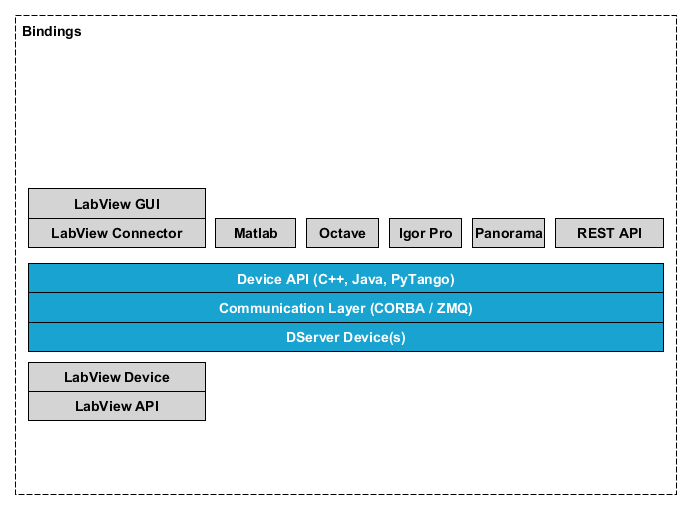
\includegraphics[width=\textwidth]{Grafika/tango_bindings_map1_1}
    \caption{Mapa wtyczek do systemu Tango Controls. Źródło: \cite{TangoDocs}.}\label{fig:tango-bindings}
\end{figure}

W związku ze wszystkimi opisanymi cechami uznano Tango Controls za odpowiednią bibliotekę do oparcia na niej części obliczeniowej aplikacji stanowiącej podstawę niniejszej pracy magisterskiej.


%-------------------------------------------------
\subsection{Architektura klasy urządzeń systemu Tango}
\label{sub:czesc-wyzsza-klasa}

Architektura systemu Tango Controls wymusiła pewne decyzje co do struktury tej części aplikacji. Zdecydowano, że będzie ona napisana jako klasa urządzeń, która określa interfejs dla wszystkich operacji wymaganych do spełnienia zadań postawionych przed tym poziomem aplikacji w podrozdziale \ref{sec:podzial-zadan}. Nie zdecydowano się na podział zadań na mniejsze klasy urządzeń komunikujące się ze sobą. Przyjęto, że prostsza struktura z jedną klasą ułatwi użycie napisanego kodu w przyszłości, np. w formie części zajęć laboratoryjnych.

\subsubsection{Interfejs dla systemu Tango}

Określając interfejs dla systemu Tango, przyjęto założenie, że wszystkie parametry statyczne modelu matematycznego powinny być również statyczną konfiguracją urządzenia, a więc należy opisać je jako jego właściwości. Głównym powodem przyjęcia takiej reguły jest fakt, iż w czasie działania - realizacji sterowania optymalnego - te wielkości nie będą się zmieniać.
Parametry dynamiczne, czyli takie, które zmieniają się między uruchomieniami algorytmów optymalizacyjnych, powinny zostać opisane jako atrybuty urządzenia.
Wszystkie dostępne akcje na modelu matematycznym zostały zaimplementowane jako komendy. Dodano tam również wszystkie akcje opisane w podrozdziale \ref{sec:komunikacja}.

Poniższa lista zawiera wszystkie istotne dla użytkownika elementy interfejsu systemu Tango urządzenia realizującego zadania wyższego poziomu aplikacji. Każdy z nich jest pokrótce opisany.

\begin{enumerate}
    \item Właściwości:
    \begin{enumerate}
        \item \emph{IPOPTTolerance} - tolerancja błędów oprogramowania do rozwiązywania zagadnień algebry liniowej (więcej o wpływie na działanie optymalizacji w sekcji \ref{sub:opt-dokladnosc}).
        \item \emph{ModelFile} - nazwa pliku z modelem dla oprogramowania do optymalizacji (więcej w sekcji \ref{sub:czesc-wyzsza-wybor}).
        \item \emph{MaxControl} - górne ograniczenie sterowania.
        \item \emph{Tank*Outflow} - opory wypływu ze zbiorników $C_{i}$. Dane jako 3 osobne właściwości - w miejscu * jest liczba 1, 2 lub 3.
        \item \emph{Tank*FlowCoeff} - współczynniki wypływu ze zbiorników $\alpha_{i}$. Dane j.w.
        \item \emph{SimulationFinalTime} - czas symulacji używanej w celu inicjalizacji algorytmu optymalizacji (więcej o tym procesie w sekcji \ref{sub:opt-init}.
        \item \emph{TCPServerEnabled} - wartość logiczna zawierająca informację o tym, czy urządzenie ma uruchomić serwer TCP w celu komunikowania się z aplikacją niższego poziomu.
        \item \emph{TCPServerAddress} - para adres i port (przedzielone dwukropkiem). Pod tym adresem serwer TCP będzie nasłuchiwał przychodzących połączeń.
    \end{enumerate}
    \item Atrybuty (nie umożliwiają zapisu, chyba że zaznaczono inaczej):
    \begin{enumerate}
        \item \emph{H*Current} - zawierają aktualne poziomy wody w zbiornikach odebrane od aplikacji niższego poziomu. Dane jako 3 osobne atrybuty - w miejscu * jest liczba 1, 2 lub 3.
        \item \emph{H*Initial} - zawierają początkowe wartości poziomów dla optymalizacji dynamicznej. Dane j.w., możliwy zapis.
        \item \emph{H*Final} - zawierają końcowe wartości poziomów dla optymalizacji dynamicznej. Dane j.w., możliwy zapis.
        \item \emph{H*Simulated} - zawierają wektory przebiegu poziomów w zbiornikach uzyskane w symulacji. Dane j.w.
        \item \emph{OptimalH*} - zawierają wektory przebiegu poziomów w zbiornikach uzyskane w czasie optymalizacji (wyznaczania sterowania czasooptymalnego). Dane j.w.
        \item \emph{OptimalTime} - liczba będąca wartością wskaźnika jakości uzyskaną w procesie wyznaczania sterowania czasooptymalnego.
        \item \emph{SimulationTime} - wektor wartości czasu uzyskany w czasie symulacji potrzebny w celu rysowania przebiegów symulacyjnych \emph{H*Simulated}.
        \item \emph{OptimalControl} - wektor zawierający sterowanie czasooptymalne.
        \item \emph{ControlCurrent} - zawiera aktualną wartość sterowania odebraną od aplikacji niższego poziomu.
        \item \emph{SwitchTimes} - wektor zawierający czasy przełączeń po normalizacji sterowania czasooptymalnego.
        \item \emph{Q} - macierz 3 na 3 zawierająca wagi poziomów do zagadnienia liniowo-kwadratowego. Możliwy zapis.
        \item \emph{R} - wartość wagi sterowania do zagadnienia liniowo-kwadratowego. Możliwy zapis.
        \item \emph{K} - wektor współczynników regulatora liniowo-kwadratowego.
        \item \emph{VerificationError} - wartość błędu weryfikacj (więcej o jego wyznaczaniu w podrozdziale \ref{sec:sym-wer}).
        \item Dostępne stany:
        \begin{enumerate}
            \item OFF - model początkowy jest niewczytany.
            \item STANDBY - model początkowy jest wczytany, ale nie trwa żadna długa operacja.
            \item ON - trwa symulacja.
            \item RUNNING - trwa optymalizacja.
            \item ALARM - długa operacja się nie udała. W przypadku optymalizacji oznacza to, iż nie udało się znaleźć sterowania optymalnego. W przypadku weryfikacji, że zwróciła ona błąd (więcej na ten temat w sekcji \ref{sub:sym-wer-jmodelica}).
        \end{enumerate}
    \end{enumerate}
    \item Komendy:
    \begin{enumerate}
        \item \emph{LoadInitialModel} - wczytuje model początkowy służący do inicjalizacji symulacji i optymalizacji.
        \item \emph{ResetModel} - resetuje wczytany model początkowy.
        \item \emph{GetEquilibriumFromControl} - przyjmuje wartość sterowania i na jej podstawie wylicza punkt równowagi, a następnie ustawia odpowiednie wartości poziomów końcowych.
        \item \emph{RunSimulation} - uruchamia symulację, a po jej zakończeniu ustawia wartości zmiennych symulacyjnych.
        \item \emph{RunVerification} - uruchamia symulację, a po jej zakończeniu ustawia wartości zmiennych symulacyjnych oraz wylicza błąd weryfikacji.
        \item \emph{Optimise} - uruchamia procedurę optymalizacji, a następnie ustawia wartości poziomów optymalnych, sterowania optymalnego i osiągniętego czasu. Przyjmuje jeden argument - wartość logiczną, która określa, czy jako wartości początkowych powinna użyć aktualnych poziomów wody w zbiornikach. Jeśli tak się dzieje, to natychmiast po zakończeniu optymalizacji uruchamia komendę \emph{SendControl}.
        \item \emph{NormaliseOptimalControl} - przeprowadza operację normalizacji sterowania czasooptymalnego (więcej na ten temat w sekcji \ref{sub:opt-dokladnosc}) i ustawia wartości czasów przełączeń.
        \item \emph{SendControl} - sprawdza, czy są gotowe wartości do wysłania do aplikacji niższego poziomu, czyli czasy przełączeń i wartości wektora $K$ (jeśli nie są gotowe, uruchamia komendę \emph{GetLQR}), a następnie wysyła je do serwera TCP.
        \item \emph{GetDataFromDirectControl} - odbiera od serwera TCP dane od aplikacji sterowania bezpośredniego. Jest odpytywana standardowo co 50 milisekund. Ustawia aktualne poziomy i sterowanie.
        \item \emph{GetLQR} - uruchamia procedurę linearyzacji i wyliczania parametrów regulatora liniowo-kwadratowego. Ustawia wartości wektora K.
        \item \emph{GetEigenvaluesFromClosedLoopWithLQR} - zwraca w formie tekstowej wartości własne macierzy $A - BR^{-1}B^{T}K$ opisującej układ zamknięty sterowany regulatorem liniowo-kwadratowym.
    \end{enumerate}
\end{enumerate}

%-------------------------------------------------
\subsection{Wybór pakietu do optymalizacji dynamicznej}
\label{sub:czesc-wyzsza-wybor}

Podstawowym elementem istotnym dla powodzenia takiego zadania był wybór pakietu realizującego operacje optymalizacji dynamicznej. Istnieje na rynku kilka płatnych bibliotek bądź pakietów oprogramowania, które są w stanie rozwiązywać tego typu problemy (np. MATLAB, Mathematica itp.), ale postanowiono poszukać darmowego odpowiednika, który posiadałby interfejs w języku programowania Python (w związku z ogólnymi założeniami co do struktury tej części aplikacji).


\subsubsection{Opis pakietu ACADO}

%TODO: definicja modelu w ACADO
Pierwszym z pakietów optymalizacyjnych, który był rozważany, jest ACADO. 


\subsubsection{Opis pakietu Modelica i \texttt{JModelica.org}}
% TODO: definicja modelu w Modelice

%-------------------------------------------------
\subsection{Środowisko testowe części obliczeniowej}
\label{sub:czesc-wyzsza-docker}
%TODO opisać Dockera
%TODO wspomnieć o budowaniu dokumentacji
